% l4h user manual.  Build with `make -C docs/manual` (needs TeX Live and
% latexmk); the PDF is a build product and is not committed.
\documentclass[11pt,a4paper]{report}

\usepackage[T1]{fontenc}
\usepackage{lmodern}
\usepackage{microtype}
\usepackage[margin=2.6cm]{geometry}
\usepackage{xcolor}
\usepackage{listings}
\usepackage{booktabs}
\usepackage{tabularx}
\usepackage{longtable}
\usepackage{enumitem}
\usepackage{tikz}
\usetikzlibrary{positioning,fit,arrows.meta}
\usepackage[hidelinks]{hyperref}

\definecolor{codebg}{gray}{0.95}
\definecolor{note}{RGB}{0,70,140}
\lstset{
  basicstyle=\ttfamily\small,
  backgroundcolor=\color{codebg},
  frame=none,
  columns=fullflexible,
  keepspaces=true,
  showstringspaces=false,
  breaklines=true,
  aboveskip=0.8em,
  belowskip=0.8em,
  xleftmargin=0.5em,
  xrightmargin=0.5em,
  upquote=true,
}
\newcommand{\cmd}[1]{\texttt{#1}}
\newcommand{\file}[1]{\texttt{#1}}
\newenvironment{caveat}{\par\medskip\noindent\color{note}\textbf{Note.}\ }{\par\medskip}
\setlist{itemsep=0.2em}
\setlength{\emergencystretch}{3em}

\title{\Huge l4h User Manual\\[0.5em]\Large A paravirtual hypervisor for Linux on seL4}
\author{The l4h project}
\date{Version 0.1 (\today)}

\begin{document}
\maketitle
\tableofcontents

%======================================================================
\chapter{Introduction}

l4h runs Linux virtual machines on the seL4 microkernel. It uses
\emph{no hardware virtualization} (no VT-x, no EL2) and emulates no
instructions. Instead, each guest runs a paravirtualized Linux kernel,
\texttt{ARCH=l4h}, derived from user-mode Linux. A guest's processes are
ordinary seL4 threads and address spaces, and its devices are virtio devices
served by host components. Because nothing depends on virtualization
extensions, l4h runs anywhere seL4 runs, including cloud VMs that do not
offer nested virtualization.

This manual is for people who build, deploy and operate an l4h host. It
covers:
\begin{itemize}
  \item building the hypervisor, the guest kernel and the tools
        (Chapter~\ref{ch:build});
  \item configuring and booting a host, on QEMU or from a UEFI disk image
        for Google Compute Engine (Chapters~\ref{ch:dom0} and~\ref{ch:boot});
  \item managing VMs, disks, switches and CPU from dom0 with \cmd{l4hctl}
        (Chapters~\ref{ch:l4hctl}--\ref{ch:cpu});
  \item recovery, troubleshooting and the test suite
        (Chapters~\ref{ch:recovery}--\ref{ch:tests}).
\end{itemize}
The design and the reasons behind it are in \file{DESIGN.md} in the source
tree, which also records the status of every part.

\section{Concepts}

\begin{description}
  \item[Host.] The machine l4h runs on: a physical machine, a QEMU VM or a
    cloud VM. It provides CPU cores, memory, PCI disks (virtio-blk or NVMe)
    and PCI NICs (virtio-net).
  \item[Guest, or VM.] A Linux system running on l4h. Every guest has a
    name, a numeric id, a number of vCPUs, a fixed amount of RAM, and up to
    16 devices: a console, disks and network interfaces.
  \item[dom0.] The first guest, id 0. It is an ordinary guest with one
    extra device, \file{/dev/l4hctl}, through which it controls the host. Its
    kernel, initramfs and settings are built into the host image. dom0 decides
    what runs, but it cannot read other guests' memory, and it runs no device
    drivers for host hardware.
  \item[Disk.] A host block device, numbered from 0 in PCI order. A disk is
    \emph{passed through} to exactly one guest, either whole or as a window
    of sectors, optionally read-only. There are no image files and no host
    filesystem.
  \item[Switch.] An L2 Ethernet switch, numbered from 0. Switches learn MAC
    addresses and flood unknown traffic. Each switch is its own broadcast
    domain.
  \item[NIC.] A host network card, numbered from 0. A NIC can be the
    \emph{uplink} of one switch: it becomes a port of that switch, and frames
    are switched to and from it like any other port.
  \item[vNIC.] A guest network interface. Each vNIC is a port on exactly one
    switch and appears in the guest as \texttt{eth}$N$.
  \item[Router VM.] l4h itself only switches Ethernet frames. Routing, NAT,
    DHCP and firewalls run in a guest of your choice, with standard Linux
    tools.
\end{description}

\section{Architecture}

Figure~\ref{fig:arch} shows the components of a running host. All of them
are seL4 user-level programs; only the seL4 kernel runs privileged.

\begin{figure}[ht]
\centering
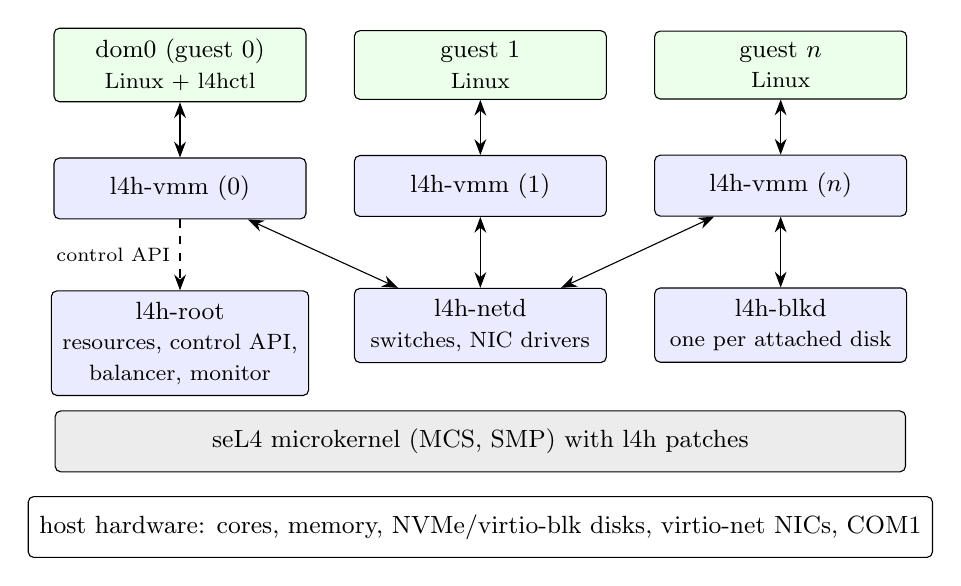
\begin{tikzpicture}[
  box/.style={draw, rounded corners=2pt, align=center, minimum height=2.2em, inner sep=4pt, font=\small},
  host/.style={box, fill=blue!8},
  guest/.style={box, fill=green!8},
  >={Stealth[length=2mm]}]
  \node[guest, minimum width=3.2cm] (dom0) {dom0 (guest 0)\\\footnotesize Linux + l4hctl};
  \node[guest, minimum width=3.2cm, right=0.6cm of dom0] (ga) {guest 1\\\footnotesize Linux};
  \node[guest, minimum width=3.2cm, right=0.6cm of ga] (gb) {guest $n$\\\footnotesize Linux};
  \node[host, below=0.7cm of dom0, minimum width=3.2cm] (v0) {l4h-vmm (0)};
  \node[host, below=0.7cm of ga, minimum width=3.2cm] (va) {l4h-vmm (1)};
  \node[host, below=0.7cm of gb, minimum width=3.2cm] (vb) {l4h-vmm ($n$)};
  \node[host, below=0.9cm of v0, minimum width=3.2cm] (root) {l4h-root\\\footnotesize resources, control API,\\\footnotesize balancer, monitor};
  \node[host, below=0.9cm of va, minimum width=3.2cm] (netd) {l4h-netd\\\footnotesize switches, NIC drivers};
  \node[host, below=0.9cm of vb, minimum width=3.2cm] (blkd) {l4h-blkd\\\footnotesize one per attached disk};
  \node[box, below=0.6cm of netd, minimum width=10.8cm, fill=gray!15] (k) {seL4 microkernel (MCS, SMP) with l4h patches};
  \node[box, below=0.3cm of k, minimum width=10.8cm] (hw) {host hardware: cores, memory, NVMe/virtio-blk disks, virtio-net NICs, COM1};
  \foreach \g/\v in {dom0/v0, ga/va, gb/vb} \draw[<->] (\g) -- (\v);
  \draw[->, dashed] (v0) -- node[left, font=\scriptsize] {control API} (root);
  \draw[<->] (v0) -- (netd); \draw[<->] (va) -- (netd); \draw[<->] (vb) -- (netd);
  \draw[<->] (vb) -- (blkd);
\end{tikzpicture}
\caption{Components of an l4h host.}
\label{fig:arch}
\end{figure}

\begin{description}
  \item[seL4] with twelve l4h patches (\file{kernel/patches}): trapping guest
    system calls, FPU state access, per-thread deadline timers and a few
    fixes.
  \item[l4h-root] is the root task. It owns all memory and devices, creates
    and destroys guests, executes control-API requests, balances vCPUs across
    cores, and runs the serial monitor.
  \item[l4h-vmm] runs once per guest. It serves the guest's hypercalls and
    virtio devices. It can map only its own guest's memory, so a compromised
    VMM can harm only that guest.
  \item[l4h-blkd] runs once per attached disk. It drives the disk (virtio-blk
    or NVMe), checks every request against the guest's memory and its sector
    window, and lets the device DMA straight into guest memory (zero copy).
  \item[l4h-netd] holds every switch and drives the uplink NICs.
\end{description}

\paragraph{Trust.} The seL4 kernel, \texttt{l4h-root}, \texttt{l4h-blkd} and
\texttt{l4h-netd} are trusted by everyone. dom0 is trusted to decide what
runs, and nothing more. Guest kernels are untrusted, and capabilities confine
them. The host does not rely on an IOMMU: the trusted drivers validate every
DMA address, and guests never touch device registers.

\section{Status and limitations}

This is version 0.1. Before you depend on it, note the following.
\begin{itemize}
  \item The Linux guest runs on x86\_64 only. On aarch64, seL4, the host
        components and a freestanding test guest run on QEMU \texttt{virt};
        the Linux guest, PCI, disks and NICs are not ported yet.
  \item The UEFI image is built for GCE N2-class machines with virtio-net,
        but it has only been tested locally, under QEMU with OVMF. gVNIC,
        which C3, C4 and N4 machines require, is not supported.
  \item There is no pause or resume, live migration, memory ballooning,
        multi-queue disks, discard, I/O rate limits or VLANs.
  \item Disk and NIC configuration is fixed when a VM is created: there is
        no hotplug.
  \item Guest RAM is reserved in full when a VM is created. Memory is not
        overcommitted, although CPU is.
\end{itemize}

%======================================================================
\chapter{Building}
\label{ch:build}

\section{Requirements}

A Linux x86\_64 build machine with:
\begin{itemize}
  \item gcc, make, cmake, ninja, git, and the Python modules seL4's build
        needs, installed in a virtual environment at \file{.venv} in the
        source tree;
  \item Rust: a stable toolchain, plus the nightly toolchain pinned in
        rust-sel4's
        \file{rust-\allowbreak toolchain.toml};
  \item the usual Linux kernel build dependencies (flex, bison, bc,
        libelf, OpenSSL headers);
  \item QEMU (\texttt{qemu-system-x86\_64}) with KVM, to run hosts locally;
  \item a static busybox, cpio and e2fsprogs, for initramfs and disk images;
  \item for UEFI images: GRUB EFI (\texttt{grub-efi-amd64-bin}), mtools,
        sfdisk and OVMF;
  \item for Debian guests: debootstrap and sudo;
  \item for aarch64: \texttt{gcc-aarch64-linux-gnu} and
        \texttt{qemu-system-arm}.
\end{itemize}
KVM serves only as a fast CPU for QEMU. The run scripts hide VMX from the
emulated machine, so seL4 runs exactly as it would on a cloud VM without
nested virtualization.

\section{Sources}

\begin{lstlisting}[language=bash]
git clone <l4h repository> l4h && cd l4h
git submodule update --init      # seL4, rust-sel4, sDDF
python3 -m venv .venv && .venv/bin/pip install sel4-deps   # seL4's build tools
\end{lstlisting}

Linux itself is not a submodule. Extract a Linux 6.18 tree into
\file{build/linux-6.18}. The build links \file{guest/linux/arch/l4h} into it
and applies the patches in \file{guest/linux/patches} once.

\section{Build steps}

\begin{longtable}{@{}p{5.2cm}p{9.3cm}@{}}
\toprule
Command & Result \\
\midrule
\endhead
\cmd{tools/build-kernel.sh} & Clones \file{kernel/seL4} into
  \file{build/seL4-src}, applies \file{kernel/patches}, builds the kernel and
  installs it with libsel4 into \file{build/sel4}. \\
\cmd{tools/build-linux.sh [targets]} & Builds the guest kernel into
  \file{build/linux-l4h} (default target \texttt{vmlinux}). On first use it
  runs \texttt{defconfig}; edit \file{build/linux-l4h/.config} or run, for
  example, \cmd{tools/build-linux.sh menuconfig} to change it. \\
\cmd{tools/build-host.sh} & Builds \texttt{l4h-vmm}, \texttt{l4h-blkd},
  \texttt{l4h-netd} and the root task \texttt{l4h-root}, which embeds them
  and the dom0 images (Chapter~\ref{ch:dom0}). The result is
  \file{host/target/\allowbreak x86\_64-sel4-roottask/\allowbreak debug/\allowbreak l4h-root.elf}. \\
\cmd{cd tools/l4hctl \&\& cargo build --release} & Builds the static
  \cmd{l4hctl} binary for dom0:
  \file{tools/l4hctl/target/release/l4hctl}. \\
\cmd{tools/mkinitramfs.sh OUT [INIT] [FILES...]} & Builds a busybox
  initramfs. \texttt{INIT} becomes \file{/init}; extra files are copied
  into \file{/bin}. \\
\bottomrule
\end{longtable}

The quickest check that everything works is the guest self-test:
\begin{lstlisting}[language=bash]
tools/build-kernel.sh
tests/run-selftest.sh 4          # builds Linux and the host, boots a 4-vCPU guest
\end{lstlisting}

\begin{caveat}
The guest kernel needs the seL4 headers, so build the kernel before Linux.
Rebuild the host (\cmd{tools/build-host.sh}) after changing dom0's
kernel, initramfs or any \texttt{L4H\_DOM0\_*} variable, since they are
embedded in \texttt{l4h-root}.
\end{caveat}

\section{Debug and release kernels}

\cmd{tools/build-kernel.sh} builds a debug seL4 kernel by default: it checks
assertions, and prints diagnostics on the serial port. For production, build
it with \texttt{L4H\_RELEASE=1 tools/build-kernel.sh}, then rebuild the host
and images. Both builds keep printing on, since the host components log
through the kernel.

seL4's debug system calls need no capability, and some of them stop the
machine. The l4h kernel reserves them to host components, so guests cannot
use them in either build.

\section{The guest kernel configuration}

\file{guest/linux/arch/l4h/configs/defconfig} gives a kernel that can boot a
general-purpose distribution: virtio-blk and virtio-net, ext4, overlayfs,
namespaces and cgroups (enough for systemd and containers), BPF, netfilter
with NAT and nftables, bridges and veth, and paravirtual steal-time
accounting, all built in. Any kernel built from
\texttt{ARCH=l4h} can serve any guest; dom0 and the other guests usually
share one \file{vmlinux}.

%======================================================================
\chapter{Configuring dom0 and the host image}
\label{ch:dom0}

An l4h host boots from two files: the seL4 kernel and \texttt{l4h-root}.
dom0's kernel, initramfs and settings are built into \texttt{l4h-root}, from
environment variables read by \cmd{tools/build-host.sh}
(Table~\ref{tab:env}).

\begin{table}[ht]
\centering
\begin{tabularx}{\linewidth}{@{}lXl@{}}
\toprule
Variable & Meaning & Default \\
\midrule
\texttt{L4H\_DOM0\_KERNEL} & dom0's kernel (an \texttt{ARCH=l4h} ELF; strip it with
  \cmd{objcopy --strip-debug} to keep the image small) & none \\
\texttt{L4H\_DOM0\_INITRD} & dom0's initramfs; empty for none & none \\
\texttt{L4H\_DOM0\_CMDLINE} & dom0's kernel command line & \texttt{console=hvc0} \\
\texttt{L4H\_DOM0\_MEM\_MB} & dom0's RAM in MiB & 256 \\
\texttt{L4H\_DOM0\_VCPUS} & dom0's vCPUs & 1 \\
\texttt{L4H\_DOM0\_DISKS} & attach the first $n$ host disks to dom0; the rest stay
  free for other guests & 64 (all) \\
\texttt{L4H\_DOM0\_NICS} & number of dom0 vNICs on switch 0 & 1 \\
\texttt{L4H\_WATCHDOG\_SECS} & print every guest's vCPU state every $n$ seconds
  (debugging); 0 disables & 0 \\
\bottomrule
\end{tabularx}
\caption{Build-time host settings.}
\label{tab:env}
\end{table}

At boot, \texttt{l4h-root}:
\begin{enumerate}
  \item finds the cores, memory, disks and NICs;
  \item creates switch 0 and makes NIC 0, if there is one, its uplink;
  \item creates dom0 with the configured disks and vNICs (dom0's vNICs are
        on switch 0, with locked MAC addresses);
  \item starts dom0 and then serves control requests.
\end{enumerate}
dom0 sees its disks as \file{/dev/vda}, \file{/dev/vdb}, \ldots{} in host
disk order, and its vNICs as \texttt{eth0}, \texttt{eth1}, \ldots

\section{A minimal busybox dom0}

dom0 needs the \cmd{l4hctl} binary and the images of the guests it will
start. A guest's image can come from anywhere dom0 can read: its initramfs,
a disk or the network. The simplest dom0 carries them in its initramfs:

\begin{lstlisting}[language=bash]
tools/build-linux.sh
objcopy --strip-debug build/linux-l4h/vmlinux build/vmlinux
(cd tools/l4hctl && cargo build --release)
tools/mkinitramfs.sh build/vm.cpio.gz          # a guest: busybox with a shell
tools/mkinitramfs.sh build/dom0.cpio.gz my-dom0-init \
    tools/l4hctl/target/release/l4hctl build/vmlinux build/vm.cpio.gz
L4H_DOM0_KERNEL=$PWD/build/vmlinux L4H_DOM0_INITRD=$PWD/build/dom0.cpio.gz \
    L4H_DOM0_MEM_MB=512 tools/build-host.sh
\end{lstlisting}

Here \file{my-dom0-init} is a shell script that becomes dom0's
\file{/init}. For example:
\begin{lstlisting}[language=bash]
#!/bin/sh
mount -t proc proc /proc
mount -t sysfs sys /sys
mount -t devtmpfs dev /dev
udhcpc -i eth0 -q
l4hctl create web --kernel /bin/vmlinux --initrd /bin/vm.cpio.gz --mem 256 --nic 0
exec /bin/sh
\end{lstlisting}

\begin{caveat}
A guest's initramfs should provide \file{/sbin/poweroff} and
\file{/sbin/reboot}. The kernel runs them when the host asks the guest to shut
down (\cmd{l4hctl shutdown}). \cmd{tools/mkinitramfs.sh} adds them.
\end{caveat}

\section{A Debian dom0}

Any distribution that runs on an x86\_64 Linux kernel can be dom0 or a guest,
as long as its kernel is an \texttt{ARCH=l4h} build. \cmd{tests/mkdebian.sh} builds
\file{build/debian.img}, a Debian 13 ext4 filesystem with systemd, a getty on
\texttt{hvc0} and DHCP on \texttt{eth0}. To boot it as dom0 from the first
host disk:

\begin{lstlisting}[language=bash]
L4H_DOM0_KERNEL=$PWD/build/vmlinux L4H_DOM0_INITRD= \
L4H_DOM0_MEM_MB=1024 L4H_DOM0_VCPUS=2 \
L4H_DOM0_CMDLINE="console=hvc0 root=/dev/vda rw" tools/build-host.sh
\end{lstlisting}
\cmd{tests/run-debian.sh} does this and boots the result under QEMU.

%======================================================================
\chapter{Booting a host}
\label{ch:boot}

\section{QEMU}

\cmd{tools/run-qemu.sh} boots seL4 and \texttt{l4h-root} directly, with
multiboot:
\begin{lstlisting}[language=bash]
tools/run-qemu.sh host/target/x86_64-sel4-roottask/debug/l4h-root.elf \
    -drive file=disk0.img,if=none,id=d0,format=raw \
    -device virtio-blk-pci,drive=d0,disable-legacy=on \
    -drive file=disk1.img,if=none,id=d1,format=raw \
    -device nvme,drive=d1,serial=d1 \
    -netdev user,id=n0 -device virtio-net-pci,netdev=n0,disable-legacy=on
\end{lstlisting}

\begin{itemize}
  \item \texttt{L4H\_SMP} (default 4) and \texttt{L4H\_MEM} (default
        \texttt{4G}) set the machine's cores and memory. Extra arguments go
        to QEMU.
  \item Disks may be \texttt{virtio-blk-pci} or \texttt{nvme}. NICs must
        be \texttt{virtio-net-pci}. Use \texttt{disable-legacy=on} for
        virtio devices. A host supports up to 4 NICs.
  \item The serial port is the console. seL4 and the host components print
        there, and so do the guests' consoles, each line prefixed with
        \texttt{[vm$N$]}. The serial monitor (Chapter~\ref{ch:recovery})
        reads it.
  \item To leave QEMU, type \texttt{Ctrl-a x}. The host never powers off by
        itself; when every guest has stopped, \texttt{l4h-root} prints
        \texttt{l4h-root: all guests stopped}.
\end{itemize}

\cmd{tools/run-dom0.sh INITRD [CMDLINE] [TIMEOUT]} combines the steps for
development. It builds Linux, embeds the given initramfs as dom0, builds the
host, and boots it with output in \file{build/qemu.log}. It stops QEMU when
all guests have stopped or after \texttt{TIMEOUT} seconds (default 60).
Extra QEMU arguments go in \texttt{L4H\_QEMU\_ARGS}.

\section{UEFI disk image}

\cmd{tools/mkimage.sh OUT.raw [l4h-root.elf]} builds a GPT disk image whose
EFI system partition holds a standalone GRUB, the seL4 kernel and
\texttt{l4h-root}. GRUB boots seL4 with multiboot2 and the serial port set
explicitly (\texttt{console\_port=0x3f8 debug\_port=0x3f8}). The size is a
whole number of GiB, as GCE requires.

To boot the image locally the way a GCE VM would (q35, OVMF, NVMe boot disk,
virtio-net):
\begin{lstlisting}[language=bash]
tools/mkimage.sh build/l4h.raw
tools/run-uefi.sh build/l4h.raw
\end{lstlisting}
The boot disk is itself an NVMe disk, so it shows up as host disk 0. Unless
you set \texttt{L4H\_DOM0\_DISKS=0}, dom0 receives it. dom0 can use the space
after the EFI partition, but it must not modify the partition itself.

\section{Google Compute Engine}

l4h has been tested on \texttt{n2-standard-4} instances: networking through
the instance's NIC, a 4-vCPU guest, a local SSD passed through to a guest and
a dozen small guests. \cmd{tests/gce-test.sh PROJECT [ZONE] [MACHINE\_TYPE]}
repeats that test: it builds an image with a test dom0, imports it, runs an
instance, prints the results from its serial port, and deletes what it
created.

\cmd{tools/gce-image.sh DISK.raw [NAME]} packages the image as GCE expects
(\file{NAME.tar.gz} containing \file{disk.raw}). It uploads nothing; it prints
the commands to run:
\begin{lstlisting}[language=bash]
gsutil cp build/NAME.tar.gz gs://BUCKET/
gcloud compute images create NAME --project=PROJECT \
    --source-uri=gs://BUCKET/NAME.tar.gz --guest-os-features=UEFI_COMPATIBLE
gcloud compute instances create NAME --project=PROJECT --zone=ZONE \
    --machine-type=n2-standard-4 --image=NAME \
    --network-interface=nic-type=VIRTIO_NET --metadata=serial-port-enable=TRUE
gcloud compute connect-to-serial-port NAME --zone=ZONE
\end{lstlisting}
Use a second-generation machine type (N2, N2D, C2) with
\texttt{nic-type=VIRTIO\_NET}: later generations offer only gVNIC. Secure
Boot must be off. l4h needs no nested virtualization.

On N2 the boot disk is attached through virtio-scsi, which l4h does not
drive: only the firmware and GRUB read it. Disks for guests are NVMe: local
SSDs (\texttt{--local-ssd=interface=NVME}), or NVMe persistent disks on
machine types that offer them.

GCE's network delivers only frames addressed to the instance's own MAC
address. dom0's first vNIC therefore takes the MAC address of the uplink
NIC, and dom0 gets the instance's address by DHCP. Put other guests on
internal switches and let dom0, or another router VM with that MAC, route
for them (Section~\ref{sec:router}).

%======================================================================
\chapter{Managing VMs with l4hctl}
\label{ch:l4hctl}

\cmd{l4hctl} is the command-line client of the control API. It runs in
dom0, where it opens \file{/dev/l4hctl}; in any other guest it fails with
\texttt{/dev/l4hctl: ... (not dom0?)}. Run it without arguments for a
summary of its commands.

All objects are named by number: VM ids from \cmd{l4hctl list}, disks from
\cmd{l4hctl disks}, NICs from \cmd{l4hctl nics}, and switches from
\cmd{switch-create}. On failure, \cmd{l4hctl} prints a reason and exits
with status 1 (Section~\ref{sec:errors}).

\section{Host information}

\begin{lstlisting}
# l4hctl info
cores:  4
memory: 2950 MiB free of 3968 MiB
disks:  2
vms:    1
# l4hctl disks
disk 0: pci 00:03.0 virtio-blk, owner vm 0
disk 1: pci 00:04.0 nvme, owner -
# l4hctl nics
nic 0: pci 00:05.0 virtio-net, uplink of switch 0
\end{lstlisting}

\section{Creating a VM}

\begin{lstlisting}
l4hctl create NAME --kernel FILE [--initrd FILE] [--mem MB] [--vcpus N]
       [--cmdline STRING] [--quota MB]
       [--disk DISK[,ro][,start=SECTOR][,sectors=N]]...
       [--nic SWITCH[,mac=MAC][,nolock]]...
\end{lstlisting}

\cmd{create} builds a VM, attaches its devices, loads its kernel and
initramfs from dom0's files and starts it. It prints the new VM's id on
standard output, and each vNIC's MAC address on standard error. If any step
fails, it destroys the half-built VM.

\begin{description}[style=nextline]
  \item[\texttt{NAME}] Up to 31 bytes, shown by \cmd{list}. Names need not
    be unique.
  \item[\texttt{--kernel FILE}] An \texttt{ARCH=l4h} kernel ELF
    (required). \cmd{l4hctl} parses it in dom0 and copies its segments into
    the guest's memory.
  \item[\texttt{--initrd FILE}] An initramfs, loaded 1 MiB above the
    kernel.
  \item[\texttt{--mem MB}] RAM, default 128 MiB. The minimum is 8 MiB; the
    maximum is 64 GiB.
  \item[\texttt{--vcpus N}] vCPUs, default 1, at most four times the host's
    cores.
  \item[\texttt{--cmdline STRING}] The kernel command line, default
    \texttt{console=hvc0}. If you replace it, keep \texttt{console=hvc0} so
    that the console works.
  \item[\texttt{--quota MB}] Memory for the guest kernel's seL4 objects:
    page tables and mapping slots of its processes. The default is
    16~MiB plus 1/16 of RAM, which suits normal workloads. Raise it for
    guests that map very large amounts of memory in many processes.
  \item[\texttt{--disk ...}] Pass a host disk through
    (Chapter~\ref{ch:storage}). Repeat it for more disks; they appear as
    \file{/dev/vda}, \file{/dev/vdb}, \ldots{} in the order given.
  \item[\texttt{--nic ...}] Add a vNIC on a switch
    (Chapter~\ref{ch:network}). Repeat it for more vNICs; they appear as
    \texttt{eth0}, \texttt{eth1}, \ldots{} in the order given.
\end{description}

A VM has at most 16 devices, counting its console.

Example: a two-vCPU web server with a disk and two networks.
\begin{lstlisting}
# sw=$(l4hctl switch-create)
# l4hctl create web --kernel /bin/vmlinux --mem 512 --vcpus 2 \
      --disk 1 --nic 0 --nic $sw --cmdline "console=hvc0 root=/dev/vda rw"
vm 1: nic on switch 0, mac 02:4c:34:00:01:01
vm 1: nic on switch 1, mac 02:4c:34:00:01:02
1
\end{lstlisting}

\section{Listing VMs}

\begin{lstlisting}
# l4hctl list
 ID NAME             VCPUS      MEM STATE
  0 dom0                 1     256M running
  1 web                  2     512M running
  2 batch                4    2048M stopped
\end{lstlisting}
A VM is \texttt{created} while it is being built, \texttt{running} once
started, and \texttt{stopped} after it powered off, rebooted or crashed. A
stopped VM keeps its memory and disks until it is destroyed. l4h does not
restart guests other than dom0; to restart one, destroy it and create it
again.

\section{The console}

Each VM has a console, \texttt{hvc0}, with an output buffer of about 16~KiB
that \texttt{l4h-root} keeps even after the VM stops.

\begin{lstlisting}
l4hctl console VM [--follow] [--until STRING] [--timeout SECS]
l4hctl send VM [--wait PATTERN [--timeout SECS]] TEXT...
\end{lstlisting}

\begin{itemize}
  \item \cmd{console VM} prints the buffered output and exits.
        \texttt{--follow} (\texttt{-f}) keeps printing new output.
        \texttt{--until STRING} stops once \texttt{STRING} has appeared,
        and \texttt{--timeout} gives up after \texttt{SECS}, with exit
        status 1. Use them in scripts to wait for a guest to come up.
  \item If output was overwritten before it was read, \cmd{console} says how
        many bytes were lost.
  \item \cmd{send VM TEXT} types \texttt{TEXT} and a newline on the
        console. With \texttt{--wait PATTERN} it then waits for
        \texttt{PATTERN} in the output (default timeout 30 s) and prints
        the round-trip time.
\end{itemize}

\begin{lstlisting}
# l4hctl console 1 --until "login:" --timeout 120 > /dev/null && echo up
# l4hctl send 1 --wait "ok" 'echo ok'
3.4 ms
\end{lstlisting}

The console of every guest is also copied to the host's serial port, which
helps when you debug a guest that dom0 cannot reach.

\section{Shutting down and destroying}

\begin{lstlisting}
l4hctl shutdown VM [--reboot]
l4hctl destroy VM
\end{lstlisting}

\cmd{shutdown} is the equivalent of pressing the power button. The guest
kernel runs \file{/sbin/poweroff} (or \file{/sbin/reboot} with
\texttt{--reboot}), so the guest's init stops its services and unmounts its
filesystems. The command returns at once; the VM's state becomes
\texttt{stopped} when it is done. A guest that reboots also stops: create it
again to restart it. Only running VMs accept \cmd{shutdown}.

\cmd{destroy} stops a VM immediately, without telling the guest, and frees
everything it held: memory, disks and vNICs. Destroying a running VM is like
pulling its power cord. To stop a VM cleanly:
\begin{lstlisting}
# l4hctl shutdown 1
# l4hctl console 1 --until "reboot: Power down" --timeout 60 > /dev/null
# l4hctl destroy 1
\end{lstlisting}
dom0 cannot destroy itself. Use the serial monitor's \texttt{restart-dom0}
for that (Chapter~\ref{ch:recovery}).

%======================================================================
\chapter{Storage}
\label{ch:storage}

\section{Disk pass-through}

A host disk is attached to one guest at a time, with the option
\begin{lstlisting}
--disk DISK[,ro][,start=SECTOR][,sectors=N]
\end{lstlisting}
whose suboptions are:

\begin{description}[style=nextline]
  \item[\texttt{ro}] The guest may read but not write; writes fail with an
    I/O error. \texttt{DISK:ro} is accepted too.
  \item[\texttt{start=SECTOR}, \texttt{sectors=N}] The guest sees only the
    window of \texttt{N} sectors from \texttt{SECTOR}, as a disk of its own
    starting at sector 0. Without \texttt{sectors}, the window extends to the
    end of the disk. Sectors are 512 bytes, as in Linux, regardless of the
    device's block size.
\end{description}

For example, to give a guest the second partition of disk 1 read-only, take
its start and size from \cmd{fdisk -l} in dom0 (while dom0 still owns the
disk) or from the partition table:
\begin{lstlisting}
# l4hctl create ro-root --kernel /bin/vmlinux \
      --disk 1,ro,start=2099200,sectors=8388608 \
      --cmdline "console=hvc0 root=/dev/vda ro"
\end{lstlisting}

\paragraph{Ownership.} A disk, including one attached as a window or
read-only, has one owner at a time. \cmd{l4hctl disks} shows the owner.
Attaching an owned disk fails with \texttt{busy}. A disk becomes free when its
owner is destroyed. Disks that dom0 received at boot stay dom0's: to make
disks available for other guests, build the host with
\texttt{L4H\_DOM0\_DISKS} set to the number dom0 should keep.

\begin{caveat}
dom0 decides which guest gets which disk, and can attach any free disk to
any guest. The host does not check what is on a disk.
\end{caveat}

\section{Performance and semantics}

Requests are checked and then sent to the device, which reads and writes
guest memory directly. Flushes reach the device, so filesystems keep their
crash-consistency guarantees. The guest sees the device's logical block
size, for example 4~KiB on 4Kn NVMe namespaces. Each disk has one queue, and
discard (TRIM) is not offered.

%======================================================================
\chapter{Networking}
\label{ch:network}

\section{Switches and uplinks}

\begin{lstlisting}
l4hctl switch-create            # prints the new switch's number
l4hctl uplink SWITCH NIC        # make host NIC the uplink of SWITCH
l4hctl switch SWITCH            # ports and counters
\end{lstlisting}

Switch 0 exists from boot and has NIC 0 as its uplink, when the host has a
NIC. Further switches are internal until you give them an uplink. A NIC can be
the uplink of one switch, and it cannot be detached. Switches cannot be
deleted; an unused switch costs nothing.

\begin{lstlisting}
# l4hctl switch 0
switch 0: uplink nic 0
PORT  VM MAC                     RX       TX  DROPS
   0   0 02:4c:34:00:00:00     1532     1611      0
   2   1 02:4c:34:00:01:02      311      290      0
\end{lstlisting}
RX and TX count frames, from the guest's point of view, and DROPS counts
frames the switch dropped for that port, for example because the guest was
not receiving, or sent a frame with another source MAC address while MAC
lock is on.

A switch remembers up to 1024 MAC addresses, forgetting each after 5
minutes without traffic. When a switch's table is full, frames from new
addresses are still delivered, by flooding.

\section{vNICs}

\texttt{--nic SWITCH[,mac=MAC][,nolock]} adds a vNIC to a new VM.

\begin{description}[style=nextline]
  \item[\texttt{mac=MAC}] The MAC address, as
    \texttt{xx:xx:xx:xx:xx:xx}. Multicast addresses are refused. By default
    the address is \texttt{02:4c:34:00:}\textit{vm}\texttt{:}\textit{port},
    a locally administered address.
  \item[\texttt{nolock}] Turn off MAC lock. By default a vNIC may send only
    frames with its own source MAC, so guests cannot impersonate each other.
    Turn it off for guests that bridge other machines, such as a Linux
    bridge or containers with their own MACs.
\end{description}

Each vNIC appears as a virtio-net device with a 1500-byte MTU. Checksum
offload and TSO pass through the switch, so guests do not compute checksums
or segment TCP for traffic that stays on the host. When a frame goes to a
port that cannot take it whole, such as a NIC without TSO or a guest that
turned the offload off, the switch segments it and computes the checksums
itself. The switch drops frames whose offload information does not match
their contents, and counts them in DROPS.

\section{A router VM}
\label{sec:router}

l4h switches frames but never routes them. To give guests on an internal
switch access to the outside, run a router VM with one vNIC on the uplink
switch and one on the internal switch. The setup below is the one
\cmd{tests/run-router.sh} checks.

In dom0:
\begin{lstlisting}
# sw=$(l4hctl switch-create)
# l4hctl create router --kernel /bin/vmlinux --mem 512 --disk 0 \
      --nic 0 --nic $sw --cmdline "console=hvc0 root=/dev/vda rw"
# l4hctl create client --kernel /bin/vmlinux --initrd /bin/vm.cpio.gz \
      --mem 128 --nic $sw
\end{lstlisting}

In the router, a Debian guest whose \texttt{eth0} gets an address by DHCP on
the uplink:
\begin{lstlisting}
sysctl -w net.ipv4.ip_forward=1
ip addr add 192.168.77.1/24 dev eth1
ip link set eth1 up
nft -f - <<'EOF'
table ip nat {
    chain postrouting {
        type nat hook postrouting priority 100;
        oifname "eth0" masquerade
    }
}
EOF
\end{lstlisting}

In the client:
\begin{lstlisting}
ip addr add 192.168.77.2/24 dev eth0
ip link set eth0 up
ip route add default via 192.168.77.1
\end{lstlisting}
The router can also run a DHCP server, a firewall or a VPN, like any Linux
router. On GCE, give the router's uplink vNIC the instance's MAC address with
\texttt{mac=}, since the VPC only delivers frames for that address.

%======================================================================
\chapter{CPU and memory}
\label{ch:cpu}

\section{Memory accounting}

Guest RAM is reserved in full when the VM is created, and returned in full
when it is destroyed. Besides its RAM, a guest uses its seL4 object quota
(\texttt{--quota}) and about 30~MiB of host objects, its VMM included. A
256~MiB guest therefore costs about 317~MiB. \cmd{l4hctl info} shows free
memory.

\texttt{l4h-root} checks every request against the memory and other kernel
resources it would need, and refuses it with \texttt{out of memory} instead
of running out. A host runs at most about 61 guests at once, dom0 included:
each guest uses 66 of the 4096 address-space identifiers seL4 has on
x86\_64.

\section{Scheduling}

vCPUs are threads that seL4 schedules by priority, with a budget for each
vCPU. Host components have priority over guests, and each guest's kernel
over guest user code, so a guest that spins cannot delay another guest's
I/O. CPU may be overcommitted: 30 guests on 4 cores work, though each gets
a share of a core.

New vCPUs are placed on cores in turn. Every 100~ms, \texttt{l4h-root}
measures how busy each vCPU was. If one core has more busy vCPUs than
another, it moves one of them to the less loaded core. It keeps a guest's
vCPUs on distinct cores where possible.

\begin{lstlisting}
l4hctl top                      # CPU use of each VM in the last 100 ms
l4hctl cores VM                 # the core each vCPU of VM runs on
l4hctl sched VM CAP             # cap each vCPU of VM at CAP% of a core
\end{lstlisting}

\begin{lstlisting}
# l4hctl top
 ID NAME               CPU%  CAP%
  0 dom0                0.4     0
  1 web                37.5     0
  2 batch             100.0    25
\end{lstlisting}
CPU\% is per VM, in percent of one core, so it can exceed 100 for a VM with
several vCPUs. CAP\% 0 means no cap.

\paragraph{CPU caps.} \cmd{l4hctl sched VM CAP} limits every vCPU of a VM to
\texttt{CAP} percent (1--100) of a core, enforced by seL4; \texttt{0} removes
the cap. A capped VM never uses more than its vCPU count times its cap, even
when cores are idle. Caps can be changed while a VM runs.

\paragraph{Steal time.} Guests see the time they were ready to run but
waiting for a core as \emph{steal}, in the \texttt{st} column of
\cmd{top} and \cmd{vmstat}, as on any cloud VM. A VM capped at 25\% that tries
to use a full core shows about 75\% steal.

%======================================================================
\chapter{Recovery and the serial monitor}
\label{ch:recovery}

\section{When dom0 fails}

If dom0 powers off, reboots or crashes, \texttt{l4h-root} destroys it and
boots it again from the host image. The other guests keep running. The new
dom0 finds them with \cmd{l4hctl list} and can manage them as before.
\texttt{l4h-root} keeps the authoritative state; dom0 needs to store
nothing to recover it. Disks and vNICs that dom0 had are recreated from the
image's settings.

\section{The dashboard}

When the host has a display and boots from the UEFI image, \texttt{l4h-root}
shows a status dashboard on the screen, refreshed every second: cores,
memory in use, every VM with its state, vCPUs, memory, CPU use, cap and
cores, the disks and their owners, and each switch with its uplink and
ports. It is read-only: there is no keyboard input. Hosts without a display,
such as GCE VMs, or booted directly by QEMU, run without it. With
\cmd{tools/run-uefi.sh}, QEMU's display shows it when you drop
\texttt{-nographic}.

\section{The serial monitor}

\texttt{l4h-root} reads commands from the host's first serial port (COM1,
which is the GCE serial console). It is the way in when dom0 is unusable.
Type a command and press Enter:

\begin{longtable}{@{}lp{10cm}@{}}
\toprule
Command & Effect \\
\midrule
\texttt{help} & list the commands \\
\texttt{list} & every VM: id, name, state, vCPUs, memory \\
\texttt{info} & cores, free and total memory, disks, NICs \\
\texttt{destroy VM} & destroy a VM other than dom0 \\
\texttt{restart-dom0} & destroy dom0 and boot it again (or boot it, if it
  is not running) \\
\bottomrule
\end{longtable}

Replies start with \texttt{monitor:}. The kernel and the guests' consoles
print to the same port, so the output may interleave. The monitor is
available only on x86\_64.

%======================================================================
\chapter{Inside a guest}
\label{ch:guest}

A guest runs an unmodified userspace on the \texttt{ARCH=l4h} kernel. From
inside, it looks like a small x86\_64 machine:
\begin{itemize}
  \item \texttt{uname -m} reports \texttt{x86\_64}, and x86\_64 binaries
        from any distribution run unchanged;
  \item the console is \texttt{hvc0};
  \item disks are \file{/dev/vda}, \file{/dev/vdb}, \ldots{} and vNICs are
        \texttt{eth0}, \texttt{eth1}, \ldots;
  \item there is no PCI, ACPI, firmware or framebuffer;
  \item time comes from the host's TSC; the wall clock starts from the
        host's real-time clock at boot (correct it with NTP as usual), and
        steal time is reported;
  \item memory protection works as on any x86\_64 machine, including
        non-executable data pages.
\end{itemize}

What does not work:
\begin{itemize}
  \item hardware virtualization, so no KVM inside a guest;
  \item device pass-through to guests other than disks.
\end{itemize}

\section{Kernel parameters}

Besides the standard ones (\texttt{root=}, \texttt{init=}, \ldots), the
guest kernel accepts:
\begin{description}[style=nextline]
  \item[\texttt{console=hvc0}] Use the l4h console. Always include it.
  \item[\texttt{earlyprintk}] Print kernel messages before the console
    driver starts.
  \item[\texttt{l4h\_strace}] Print every system call of every process.
    Very verbose; for debugging the guest kernel.
  \item[\texttt{l4h\_debug\_user}] Print the faults and exceptions of user
    processes.
\end{description}

%======================================================================
\chapter{Troubleshooting}
\label{ch:trouble}

\section{l4hctl errors}
\label{sec:errors}

\begin{longtable}{@{}p{4.3cm}p{10.2cm}@{}}
\toprule
Message & Usual cause \\
\midrule
\endhead
\texttt{/dev/l4hctl: ... (not dom0?)} & \cmd{l4hctl} runs in a guest other
  than dom0, or dom0's kernel lacks the l4hctl driver. \\
\texttt{no such VM or device} & The VM, disk, NIC or switch number does not
  exist. \\
\texttt{out of memory} & The host lacks the memory, or another kernel
  resource, for the request. See \cmd{l4hctl info}; destroy stopped VMs,
  which still hold their memory. When free memory is fragmented, a large VM
  can fail even though \cmd{info} shows enough. \\
\texttt{busy} & The disk already has an owner; the VM is not in the right
  state, for example \cmd{shutdown} on a stopped VM, or devices added
  after the VM started. \\
\texttt{invalid argument} & Out-of-range values: 0 or too many vCPUs, RAM
  below 8 MiB, a cap above 100, a multicast MAC, a kernel that does not fit in the VM's RAM, or a request
  that targets dom0 itself. \\
\texttt{no space for devices} & The VM already has 16 devices. \\
\texttt{operation not permitted} & dom0 tried to destroy itself. \\
\texttt{not a 64-bit little-endian ELF} & \texttt{--kernel} does not name a
  kernel ELF; pass \file{vmlinux}, not a compressed image. \\
\bottomrule
\end{longtable}

\section{Common problems}

\begin{description}[style=nextline]
  \item[Nothing appears on the serial port after GRUB.] seL4 must be told
    the serial port on UEFI systems. Use the images from
    \cmd{tools/mkimage.sh}, which pass \texttt{console\_port=0x3f8}.
  \item[The guest console stays empty.] Check that the command line
    contains \texttt{console=hvc0}. Guest output is also copied to the host
    serial port with a \texttt{[vm$N$]} prefix; look there for early boot
    messages, adding \texttt{earlyprintk} if needed.
  \item[\cmd{l4hctl shutdown} has no effect.] The guest lacks
    \file{/sbin/poweroff}, or its init ignores the request. Busybox and
    systemd handle it; a custom \file{/init} must not ignore SIGTERM or
    must run \file{/sbin/poweroff} itself. Use \cmd{destroy} as a last
    resort.
  \item[A guest has no network.] Check with \cmd{l4hctl switch} that its
    vNIC is on the intended switch and that the switch has an uplink or a
    router. If a guest bridges other MACs, create its vNIC with
    \texttt{nolock}.
  \item[Guests feel slow.] Use \cmd{l4hctl top} to find busy VMs and
    \cmd{l4hctl sched} to cap them. Steal time inside a guest shows how much
    it waits for a core. On a host that is itself a nested VM, every
    cross-core wake-up is expensive, which hurts network latency.
  \item[A guest panics in its kernel.] Its console holds the panic message
    (\cmd{l4hctl console VM}). Rebuilding the host with
    \texttt{L4H\_WATCHDOG\_SECS} set prints every vCPU's registers
    periodically, which helps with hangs.
\end{description}

%======================================================================
\chapter{Tests}
\label{ch:tests}

The integration tests boot hosts in QEMU and print \texttt{PASS} or
\texttt{FAIL}. They need KVM and about 4~GiB of free memory; the density test
needs 16~GiB. The Debian tests need \cmd{tests/mkdebian.sh} to have run once.

\begin{longtable}{@{}p{5.6cm}p{8.9cm}@{}}
\toprule
Test & What it checks \\
\midrule
\endhead
\cmd{run-testguest.sh},\newline\cmd{run-testguest-aarch64.sh} & the guest ABI
  and seL4 extensions, with a freestanding guest \\
\cmd{run-selftest.sh [vcpus]} & system calls, memory, signals, fork,
  threads, futexes, SMP stress \\
\cmd{run-blktest.sh} & disk pass-through and data integrity
  (\texttt{BLKTEST\_DEV=nvme} for NVMe) \\
\cmd{run-ctltest.sh} & VM lifecycle, console, clean shutdown, disk windows,
  memory reclaim \\
\cmd{run-nettest.sh} & DHCP over the uplink, switches, several vNICs,
  isolation, MAC lock \\
\cmd{run-router.sh} & a Debian NAT router VM between an internal switch and
  the uplink \\
\cmd{run-density.sh 30 256} & 30 guests of 256 MiB on 4 cores stay
  responsive \\
\cmd{run-m6test.sh} & dom0 restart, CPU caps, steal time \\
\cmd{run-limits.sh} & the host refuses what it cannot afford and recovers \\
\cmd{run-monitor.sh} & the serial monitor \\
\cmd{run-uefitest.sh} & the UEFI image with NVMe boot disk and virtio-net,
  as on GCE \\
\cmd{run-debian.sh}, \cmd{run-workload.sh} & Debian with systemd, fio
  verification, a parallel build, fsck, data surviving a reboot \\
\cmd{run-bench.sh} & micro-benchmarks \\
\cmd{run-fuzz.sh} & a hostile guest fuzzing the VMM's virtqueues \\
\bottomrule
\end{longtable}

%======================================================================
\appendix
\chapter{Limits}

\begin{longtable}{@{}lr@{}}
\toprule
Limit & Value \\
\midrule
Host cores & 64 \\
Host disks & 64 \\
Guests per host, including dom0 & about 61 (64 ids) \\
vCPUs per guest & $4\times$ host cores, at most 64 \\
RAM per guest (in at most 128 contiguous chunks) & 8 MiB to 64 GiB \\
Devices per guest (console, disks, vNICs) & 16 \\
Host NICs & 4 \\
Switch ports, all switches together & 48 \\
Learned MAC addresses & 1024 per switch, 8192 in all \\
Guest name & 31 bytes \\
Kernel command line & 1983 bytes \\
Console output buffer per guest & about 16 KiB \\
\bottomrule
\end{longtable}

\chapter{Control API reference}

\cmd{l4hctl} is a thin client; other dom0 programs can use the control API
directly. \file{/dev/l4hctl} takes one ioctl, \texttt{\_IOWR('L', 1, struct
l4hctl\_call)}, whose argument points to a request, a response and, for
\texttt{VM\_LOAD}, a data buffer. The structures are defined in
\file{include/l4h/abi.h}:
\begin{itemize}
  \item a request has an operation, the ABI version (1), six 64-bit
        arguments and 1984 bytes of data;
  \item a response has a status (0 or a negative errno), six 64-bit values
        and 1984 bytes of data.
\end{itemize}
Requests run synchronously, one at a time.

\begin{longtable}{@{}r>{\raggedright\arraybackslash}p{3.6cm}>{\raggedright\arraybackslash}p{4.6cm}>{\raggedright\arraybackslash}p{4.7cm}@{}}
\toprule
Op & Name & Arguments & Results \\
\midrule
\endhead
1 & \texttt{HOST\_INFO} & -- & cores, free bytes, total bytes, disks, VMs,
  NICs \\
2 & \texttt{VM\_CREATE} & RAM bytes, vCPUs, guest RAM base, quota bytes;
  name in data & VM id \\
3 & \texttt{VM\_LOAD} & VM, guest-physical address; bytes in the buffer
  (at most 4 MiB) & -- \\
4 & \texttt{VM\_START} & VM, entry point, end of kernel, initrd address,
  initrd size; command line in data & -- \\
5 & \texttt{VM\_DESTROY} & VM & -- \\
6 & \texttt{VM\_LIST} & first VM id & count; \texttt{struct l4h\_ctl\_vm}
  entries in data \\
7 & \texttt{BLK\_ATTACH} & VM, disk, read-only, first sector, sectors & -- \\
8 & \texttt{CONSOLE\_READ} & VM, offset & next offset, bytes, bytes lost;
  output in data \\
9 & \texttt{CONSOLE\_WRITE} & VM, length; input in data & bytes accepted \\
10 & \texttt{DISK\_INFO} & disk & PCI address, owner (or $2^{64}-1$), --,
  kind (0 virtio-blk, 1 NVMe) \\
11 & \texttt{SWITCH\_CREATE} & -- & switch \\
12 & \texttt{SWITCH\_ATTACH\_\allowbreak UPLINK} & switch, NIC & -- \\
13 & \texttt{NIC\_CREATE} & VM, switch, MAC (0: default), flags (1: no MAC
  lock) & MAC \\
14 & \texttt{SWITCH\_INFO} & switch & ports, uplink NIC; \texttt{struct
  l4h\_ctl\_port} entries in data \\
15 & \texttt{NIC\_INFO} & NIC & PCI address, switch (or $2^{64}-1$) \\
16 & \texttt{VM\_SET\_SCHED} & VM, cap percent & -- \\
17 & \texttt{VM\_INFO} & VM & host core of vCPUs 0--5 \\
18 & \texttt{VM\_STATS} & VM & CPU use in tenths of a percent, cap \\
19 & \texttt{VM\_SHUTDOWN} & VM, 0 power off / 1 reboot & -- \\
\bottomrule
\end{longtable}

A VM is built in this order: \texttt{VM\_CREATE}, then any
\texttt{BLK\_ATTACH}, \texttt{NIC\_CREATE} and \texttt{VM\_LOAD} requests,
then \texttt{VM\_START}. Devices and images can only be added before the VM
starts. The host never parses guest images: the client loads the kernel's
segments to their addresses relative to the RAM base it passed to
\texttt{VM\_CREATE}, and names the entry point in \texttt{VM\_START}.

\end{document}
